\documentclass[final,hyperref={pdfpagelabels=false}]{beamer}
\usepackage{grffile}
\mode<presentation>{\usetheme{ECOMP}}
%\usepackage[portuges, brazil]{babel}   
\usepackage[utf8]{inputenc}
\usepackage{amsmath,amsthm, amssymb, latexsym}
%\usepackage{times}\usefonttheme{professionalfonts}  % obsolete
%\usefonttheme[onlymath]{serif}
\boldmath
\usepackage[orientation=portrait,size=a1,scale=1.4,debug]{beamerposter}
% change list indention level
% \setdefaultleftmargin{3em}{}{}{}{}{}


%\usepackage{snapshot} % will write a .dep file with all dependencies, allows for easy bundling

\usepackage{array,booktabs,tabularx}
\newcolumntype{Z}{>{\centering\arraybackslash}X} % centered tabularx columns
\newcommand{\pphantom}{\textcolor{ta3aluminium}} % phantom introduces a vertical space in p formatted table columns??!!

\listfiles

%%%%%%%%%%%%%%%%%%%%%%%%%%%%%%%%%%%%%%%%%%%%%%%%%%%%%%%%%%%%%%%%%%%%%%%%%%%%%%%%%%%%%%
\graphicspath{{figures/}}
 
\title{\huge Desenvolvimento de um poster para o E-Comp, com os logos que tem geometrias diferentes}
\author{Alessandro Camillo Gimenez de Menezes\inst{1} Ezequiel França dos Santos\inst{1}, Gabriel Vieira Figueiredo Tomaz\inst{1}}
\institute[SENAC]{Centro Universitário Senac - Campus Santo Amaro}
\date[Dezembro 3th, 2014]{Dezembro 03, 2014}

%%%%%%%%%%%%%%%%%%%%%%%%%%%%%%%%%%%%%%%%%%%%%%%%%%%%%%%%%%%%%%%%%%%%%%%%
\newlength{\columnheight}
\setlength{\columnheight}{105cm}
%%%%%%%%%%%%%%%%%%%%%%%%%%%%%%%%%%%%%%%%%%%%%%%%%%%%%%%%%%%%%%%%%%%%%%%%
\begin{document}%Inicia o documento
\begin{frame}
  \begin{columns}%Inicia as Colunas
    % ---------------------------------------------------------%
    % Configurar a primeira coluna
\begin{column}{.49\textwidth}
      \begin{beamercolorbox}[center,wd=\textwidth]{postercolumn}
        \begin{minipage}[T]{.95\textwidth} % tweaks the width, makes a new \textwidth
          \parbox[t][\columnheight]{\textwidth}{ % must be some better way to set the the height, width and textwidth simultaneously
            % Since all columns are the same length, it is all nice and tidy.  You have to get the height empirically
            % ---------------------------------------------------------%
            % fill each column with content
            
            %%RESUMO%%%%%%%%%%%%%%%%%
           \color{blue} % Navy color for the abstract

\begin{abstract}

Biodiversity, the term used to describe the wide variety of species on Earth, is declining at enormous rates due to human-induced environmental changes. This compromises ecosystem stability and productivity, which negatively impacts the ecosystem services that support life on Earth.

The mechanisms that control the diversification of species are poorly understood. In the last decade sophisticated diversification models have been developed, but these models ignore ecological interactions. While current models have examined factors such as competition, predator-prey interactions, parasitism, and mutualism, they have been developed on a case-by-case basis, and no general method to study the combined effect of these factors exists.

Such a general method has remained elusive for several reasons. Firstly, evolutionary processes have extremely complex dynamics. Secondly, decay and fossilization degrade crucial evidence useful for phylogenetic analyses that could infer underlying mechanisms. Thirdly, diversification processes have many potential explanatory variables, which increases the dimensionality of the models enormously.

To overcome these issues, we propose a general speciation model with potentially many covariates. This complex stochastic differential equation model can be written equivalently as a combination of two generalized linear models. The fact that we typically only have data on currently existing species can be described as a missing data problem. For sparse inference of the speciation parameters we integrate sparse stochastic approach by integrating a sequential path estimator in the M-step of the EM algorithm.
% We make use of the underlying differential geometry of the speciation models results using a sparse, computationally feasible and consistent model selection procedure (dDgLARSlars). The dDgLARSlars algorithm has been successfully applied in the context of sparse generalized linear models, but their application to diversification models is a novel methodological contribution. 

%We show that our model has the potential to select the ecological factors that are key to driving species diversification.

\end{abstract}
            %\vfill
            %%INTRODUÇÃO%%%%%%%%%%%%%
            \section*{Materials and Methods}
            Consider 
            $$ E(llik(\theta)) \propto  l(\theta)=\displaystyle\sum_{j=1}^{N_j} l(\theta | s_j) $$
           % \vfill
            %%%%%%%%%%OBJETIVOS%%%%%%%%%%%%%%
            \begin{block}{Objetivos}
             Este trabalho apresenta a proposta de um sistema de visualização de dados, seguindo uma arquitetura de web crawler - web service - visualização. 
             
Neste trabalho, para o obtenção dos dados foi utilizada uma técnica de crawling 
		
            \end{block}
        	%\vfill    
            %%%%%%%%%%%%%METODOLOGIA%%%%%%%%
            \begin{block}{Metodologia}
              \begin{itemize}
              \item Grid-based local feature extraction instead of interest points
              \item Local descriptors:
                \begin{itemize}
                \item upright descriptor versions achieved better results
                \item SURF-128 better than SURF-64
                \end{itemize}
              \item System robustness: manually aligned/unaligned/partially occluded faces
                \begin{itemize}
                \item SURF more robust to illumination
                \item SIFT more robust to changes in viewing conditions
                \end{itemize}
              \item RANSAC-based system combination and outlier removal
              \end{itemize}
              Lorem Ipsum é simplesmente uma simulação de texto da indústria tipográfica e de impressos, e vem sendo utilizado desde o século XVI, quando um impressor desconhecido pegou uma bandeja de tipos e os embaralhou para fazer um livro de modelos de tipos. Lorem Ipsum sobreviveu não só a cinco séculos, como também ao salto para a editoração eletrônica, permanecendo essencialmente inalterado. Se popularizou na década de 60, quando a Letraset lançou decalques contendo passagens de Lorem Ipsum, e mais recentemente quando passou a ser integrado a softwares de editoração eletrônica como Aldus PageMaker.
            \end{block}
            \vfill
          }
          % ---------------------------------------------------------%
          % end the column
        \end{minipage}
      \end{beamercolorbox}
    \end{column}
    % ---------------------------------------------------------%
    % Fim da coluna 1

    % ---------------------------------------------------------%
    % Ajuste da Coluna 2
    \begin{column}{.49\textwidth}
      \begin{beamercolorbox}[center,wd=\textwidth]{postercolumn}
        \begin{minipage}[T]{.95\textwidth} % tweaks the width, makes a new \textwidth
          \parbox[t][\columnheight]{\textwidth}{ 
            \begin{block}{Databases}
              \begin{columns}
                \begin{column}{.6\textwidth}
                  \begin{itemize}
                  \item AR-Face 
                    \begin{itemize}
                    \item variations in illumination
                    \item many different facial expressions
                    \end{itemize}
                  \item CMU-PIE
                    \begin{itemize}
                    \item variations in illumination (frontal images from the illumination subset)
                    \end{itemize}
                  \end{itemize}
                \end{column}
                \begin{column}{.39\textwidth}
                  
\includegraphics[width=0.22\linewidth]{hanselmann-databases/arface/train/png/occlusions/arneutral/m-016-1}
                  \-
                  
\includegraphics[width=0.22\linewidth]{hanselmann-databases/arface/train/png/cropped/m-016-4}
                  \-
                  
\includegraphics[width=0.22\linewidth]{hanselmann-databases/arface/test/png/occlusions/ar1sun/m-016-8}
                  \-
                  
\includegraphics[width=0.22\linewidth]{hanselmann-databases/arface/test/png/occlusions/ar1scarf/m-016-11}
                  \vskip3ex

                  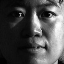
\includegraphics[width=0.22\linewidth]{hanselmann-databases/cmupie/test/png/cropped/00-27-02}
                  \-
                  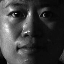
\includegraphics[width=0.22\linewidth]{hanselmann-databases/cmupie/test/png/cropped/00-27-17}
                  \-
                  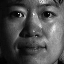
\includegraphics[width=0.22\linewidth]{hanselmann-databases/cmupie/test/png/cropped/00-27-18}
                  \-
                  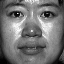
\includegraphics[width=0.22\linewidth]{hanselmann-databases/cmupie/test/png/cropped/00-27-20}
                \end{column}
              \end{columns}
            \end{block}
            \vfill
            
            %%%%
            \begin{block}{Results: Manually Aligned Faces}
              \begin{itemize}
              \item AR-Face: 110 classes, 770 train, 770 test
              \end{itemize}
              \vskip-0.5ex
              \begin{table}
                \centering
                \small
                \begin{tabular}{@{} p{.2\linewidth} p{.18\linewidth} p{.25\linewidth} r r r @{}}
                  \toprule 
                  Descriptor &  Extraction        & \multicolumn{1}{p{.2\linewidth}}{\# Features}           & \multicolumn{3}{c @{}}{Error Rates [\%]}         \\
                  \cmidrule(l){4-6}
                             &                    &                                                      & \multicolumn{1}{c}{Maximum} & \multicolumn{1}{c}{Grid} & \multicolumn{1}{c @{}}{Grid-Best} \\
                  \cmidrule(r){1-1}  \cmidrule(lr){2-2}   \cmidrule(lr){3-3}                               \cmidrule(lr){4-4}            \cmidrule(lr){5-5}         \cmidrule(l){6-6}  
                  SURF-64    & IPs                & \pphantom{1}64 $\times$ 5.6 (avg.)                    & 80.64     &  84.15  & 84.15     \\
                  SIFT       & IPs                & 128 $\times$ 633.78 (avg.)                           & 1.03      &  95.84  & 95.84      \\
                  \addlinespace
                  SURF-64    & 64x64-2 grid       & \pphantom{1}64 $\times$ 1024                          & 0.90      &  0.51   & 0.90      \\  
                  SURF-128   & 64x64-2 grid       & 128 $\times$ 1024                                    & 0.90      &  0.51   & 0.38       \\
                  SIFT       & 64x64-2 grid       & 128 $\times$ 1024                                    & 11.03     &  0.90   & 0.64       \\
                  \addlinespace
                  U-SURF-64  & 64x64-2 grid       & \pphantom{1}64 $\times$ 1024                          & 0.90      &  1.03   & 0.64      \\ 
                  U-SURF-128 & 64x64-2 grid       & 128 $\times$ 1024                                    & 1.55      &  1.29   & 1.03       \\ 
                  U-SIFT     & 64x64-2 grid       & 128 $\times$ 1024                                    & \textbf{0.25}  &  \textbf{0.25}   & \textbf{0.25}  \\
              
                  \bottomrule
                \end{tabular}
              \end{table} 
            \end{block}
            \vfill
            

            \begin{block}{Conclusão}
              O trabalho apresenta como principal contribuição, uma possibilidade de reconhecimento de padrões pré-determinados  para controle de jogos utilizando métodos simples, porém com resultados, dentro de seus limites, precisos.

Os algoritmos propostos são de fácil implementação e não requerem uma abordagem matemática profunda para sua compreensão e aplicação. O trabalho mostra ainda, que estes métodos, com pouca modificação poderiam ser utilizados em qualquer outro tipo de interface por visão computacional, uma vez que seus algoritmos possuem complexidades relativamente médias.
%%% References
            \end{block}
            \vfill
            \begin{block}{Referencias Bibliograficas}
              \begin{itemize}
              \item Eu nao me preocupei com acentos e etc, logo, verifique 
              \item Misturar paçoquita cremosa com Nutella é bem legal
              \item LEMBRE-SE DO VFILL, SE VAI USAR OU NAO EM CADA BLOCO.
              \end{itemize}
            \end{block}
            \vfill
          }
           
          % ---------------------------------------------------------%
          % end the column
        \end{minipage}
      \end{beamercolorbox}
    \end{column}
    % ---------------------------------------------------------%
    % end the column
  \end{columns}
  \vskip1ex
\end{frame}
\end{document}


%%%%%%%%%%%%%%%%%%%%%%%%%%%%%%%%%%%%%%%%%%%%%%%%%%%%%%%%%%%%%%%%%%%%%%%%